\section{Sobre o projeto}

A solução apresentada consiste em um repositório template do Github  que se converte em um ambiente de desenvolvimento que podemos chamar de Devcontainer. Apesar do nome, não  há necessidade alguma de conhecimento em programação e possui as seguintes funcionalidades:

\begin{itemize}
	\item Colaborativo: Utiliza 100\% de ferramentas do github para escrever artigos com orientadores e outros autores.
	\item Simples mas completo: Basta clonar e editar os textos. Com um conhecimento básico de LaTex que o próprio repositório fornecem nas instruções iniciais já é possível escrever um artigo completo, mas é util também para pessoas com o conhecimento avançado em LaTex.
	\item Online e Offline: Você pode utilizar o navegador para editar, mas é possivel acessar de forma offline também.
\end{itemize}


As edições podem ocorrer de três formas: diretamente no github pelo repositório, de forma online pelo github (figura~\ref{fig:fig01}), pela plataforma codespaces (figura~\ref{fig:fig02}), ou de forma offline pelo Visual Studio Code (figura~\ref{fig:fig03}).


\begin{figure}[ht]
	\centering
	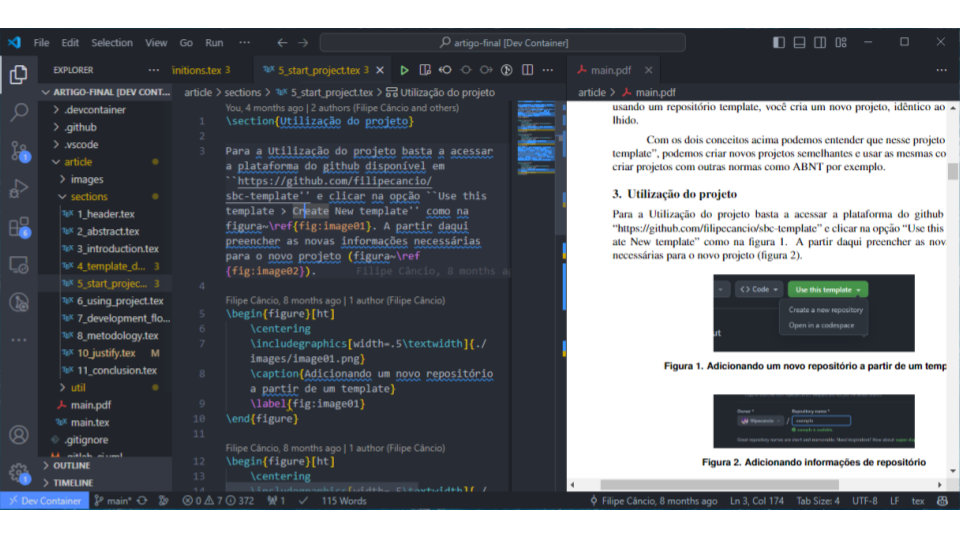
\includegraphics[width=.6\textwidth]{./images/fig01.png}
	\caption{Utilizando o projeto no site do GitHub}
	\label{fig:fig01}
\end{figure}

\begin{figure}[ht]
	\centering
	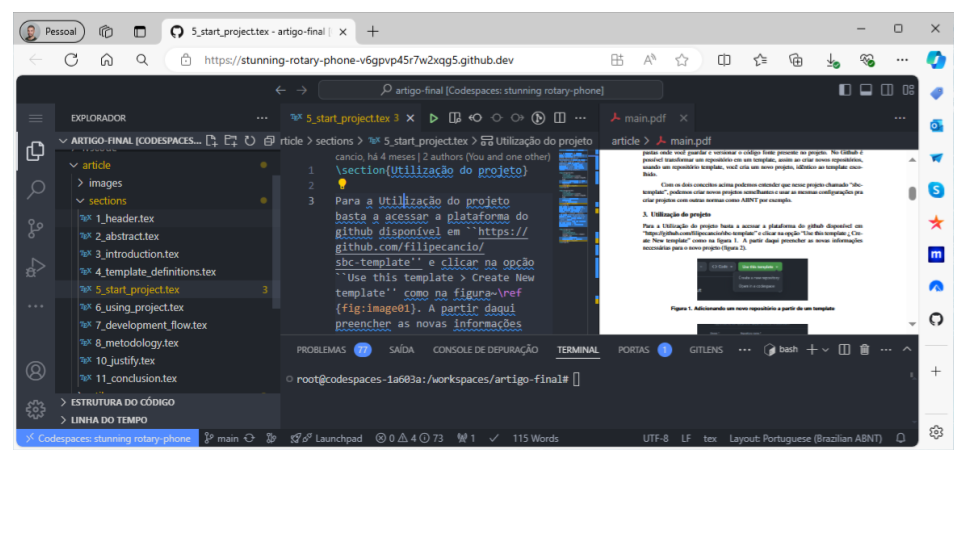
\includegraphics[width=.6\textwidth]{./images/fig02.png}
	\caption{Utilizando o projeto pelo Codespaces}
	\label{fig:fig02}
\end{figure}

\begin{figure}[ht]
	\centering
	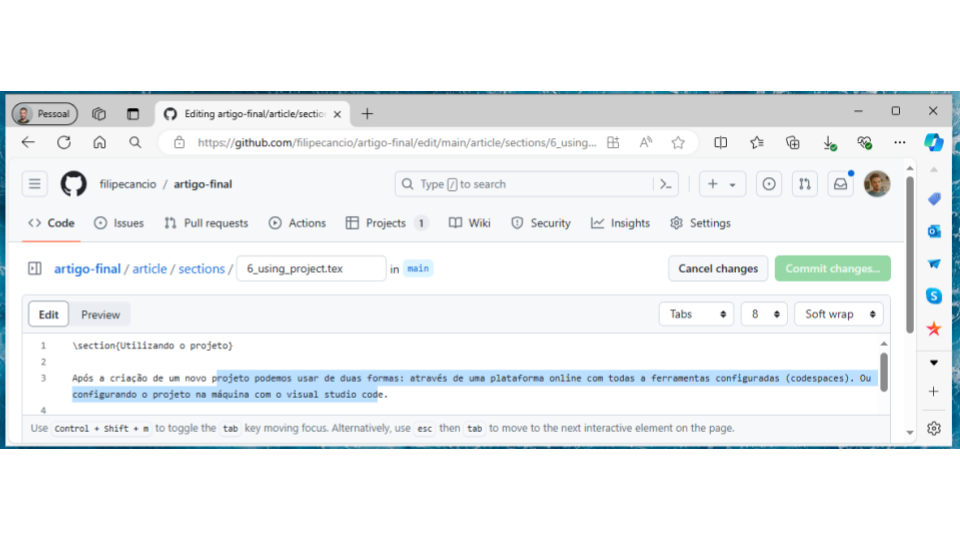
\includegraphics[width=.6\textwidth]{./images/fig03.png}
	\caption{Utiizando o projeto com Visual Studio Code}
	\label{fig:fig03}
\end{figure}

\subsection{Vantagens do projeto}

\subsubsection{Versões de release}
Considerando que o projeto utiliza 100\% de ferramentas do github, uma das funcionalidades mais marcantes é a geração de arquivos .pdf de forma automática associada ao controle de versão Git. A cada nova edição, o repositório gera um novo pdf com as alterações realizadas. A cada commit gerado na banch de ``main'' é gerada uma versão de release com o pdf datado (imagem~\ref{fig:fig04}). Essa funcionalidade descarta qualquer necessidade de salvar versões de pdf, uma vez que o github tem tudo salvo e documentado.

\begin{figure}[ht]
	\centering
	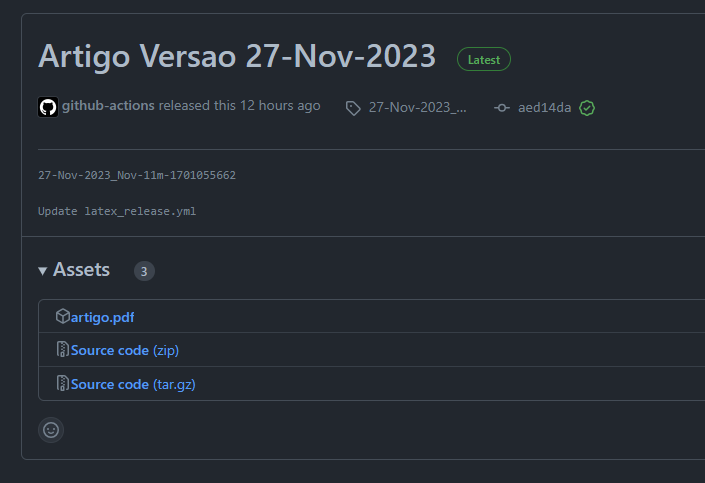
\includegraphics[width=.6\textwidth]{./images/fig04.png}
	\caption{Detalhes da ultima release}
	\label{fig:fig04}
\end{figure}

\subsubsection{Pull Requests}

Os artigos não precisam ser desenvolvidos na ramificações ``main''. O manual de instruções do projeto orienta que o pesquisador deve criar novas ramificações para implementar novos tópicos e correções, associado a isso, pode ser utilizada a ferramenta de Pull Requests do GitHub para promover entre autor e orientador o controle das mudanças em cada versão, facilitando a corressaum dos artigos.
